\documentclass[runningheads]{llncs}

\usepackage{graphicx}
\usepackage{amsmath}
\usepackage{amssymb}
\usepackage{booktabs}

\begin{document}

\title{Project Report on Ant Colony Optimization applied to the Permutation Flow Shop Problem with Weighted Tardiness}

\titlerunning{Project Report on ACO applied to the PFSP-WT}

\author{Théo Verhelst}

\institute{Université Libre de Bruxelles}

\maketitle

\begin{abstract}

This report describes our work on the final assignment of the \emph{INFO-F414
Swarm Intelligence} course. This assignment concerns the evaluation of different
Ant Colony Optimization (ACO) algorithms applied to the \emph{Permutation Flow
Shop Problem} with \emph{Weighted Tardiness}. We implemented two variants of the
Ant System algorithm, namely the \emph{ranked-based} variant and the
\emph{Max-Min} variant \cite{stutzle1998ant}. We also implemented the
\emph{Greedy Iterative Random Local Search} \cite{karabulut2016hybrid}. The
algorithm parameters have been optimized using a grid search procedure, and the
performance of the three algorithms are compared. We use 20 instances of the
permutation flow shop problems given in \cite{taillard1993benchmarks}.

\end{abstract}

\section{Introduction}

This report presents the work we conducted for the final assignment of the
\emph{INFO-F414 Swarm Intelligence} course.

The rest of this report is organized as follow: section \ref{sec:prob} presents
the permutation flow shop problem with weighted tardiness in a formal manner.
Section \ref{sec:algo} describes in details the three algorithms we used to
solve the problem, the local search approach, as well as the representation
chosen for the different data structures. Section \ref{sec:exp} presents the
experiments we conducted for optimizing and assessing the performance of the
three algorithms and the local search. The results are shown and discussed in
section \ref{sec:res}. Finally, a conclusion is given in section
\ref{sec:conclusion}.

\section{Problem description}
\label{sec:prob}

The permutation flow shop problem consists in scheduling a set of of $n$ jobs.
Each job needs to be executed on $m$ different machines in order. Each job
$i\in N = \{1,\dots,n\}$ needs a non-negative execution time $p_{i,j}$ on machine
$j\in M = \{1,\dots, m\}$. The objective is to find a permutation of the set
$\{1,\dots,n\}$ representing the order in which the jobs are scheduled, as to
minimize some objective function. The completion time $C_{i,j}$ is the total
time needed to complete the execution of job $i$ on machine $j$, and is defined
as

\begin{equation}
	C_{i,j}=\max(C_{i-1,j}, C_{i, j-1}) + p_{i,j}\quad\forall i\in N,j\in M.
\end{equation}

That is, the jobs starts its execution on a machine either when it finishes its
execution on the previous machine, or when the previous jobs is done with the
machine, whichever happens first. The first job starts on the first machine
without delay, which is formally defined as $C_{i, 0} = 0$ and $C_{0, j} = 0$,
for all $i\in N$ and $j\in M$. Each jobs $i$ has an associated non-negative due
date $d_i$, which indicates the time at which the job should have finished its
execution on the last machine. This allows to define the \emph{tardiness}
$T_i=\max(0, C_{i, m} - d_i)$. A different weight $w_i$ is given to each job,
and the \emph{total weighted tardiness} is thus defined as $\sum_{i=1}^n
w_iT_i$. Our objective in this project is to find a permutation $\pi$ of the $n$
jobs that minimizes the total weighted tardiness $f(\pi)$. This definition of
the problem implies that

\begin{itemize}
	\item all jobs are ready to be executed at instant 0;
	\item all machines are always available;
	\item a job can execute on one machine at a time;
	\item the job order is the same for all machines;
	\item no preemption is allowed.
\end{itemize}


\section{Algorithms description}
\label{sec:algo}

We implemented three different search algorithms. Two are variants of the Ant
System, and one is an iterated search. All of these three algorithms start by
using the NEH-edd heuristic \cite{kim1993new}, which is itself an adaptation for
tardiness of the NEH heuristic \cite{nawaz1983heuristic}. We in turn modified it
as to take into account the weighted total tardiness instead of the total
tardiness as evaluation measure. In the case of the two ant systems, this
initial solution is used to initialize the trail, whereas it used as the
starting point of the iterated search approach. The NEH-edd heuristic consists
in sorting all jobs by increasing due date, and iteratively inserting jobs at
the best position among the scheduled jobs. At iteration $i\in N$, the job $i$
in the sorted list of jobs is considered for insertion in the partial solution
between all positions $j$ and $j+1$, for $j\in\{1,\dots,i\}$. The insertion that
yields the least weighted total tardiness is chosen, the job is inserted, and
the next iteration begins. This stops when all jobs are scheduled. This
heuristic requires the ability to evaluate solutions that do not schedule the
entire set of $n$ jobs.

\subsection{Rank-based Ant System}

The first variant of Ant System is the Rank-based Ant System (RB-AS), inspired
from the course material. The solutions are constructed by each ant based solely
on the pheromone trail, in an iterative manner. For each position $j\in N$, a
job is chosen amongst the set yet unscheduled jobs $N'$, according to a discrete
probability density whose terms are proportional to $\tau_{i,j}\;\forall i\in
N'$. At the end of each iteration, a number $\omega$ of ants with the best
iteration solutions are selected for updating the trail. The trail at iteration
$t$ is updated as

\begin{equation}
	\label{update_rank_based}
	\tau_{i,j}(t)=\rho\tau_{i,j}(t-1)+\sum_{r=1}^\omega(\omega-r-1)\Delta\tau_{i,j}^{(r)}
\end{equation}
where $\tau_{i,j}(t)$ denotes the willingness of an ant to place job $j$ at position
$j$ in the solution, $\rho$ is the trail persistence parameter, and

\begin{equation}
	\Delta\tau_{i,j}^{(r)}=
		\begin{cases}
			1/f(\pi_r)\quad&\text{if job }i\text{ is }j\text{th position in the solution of ant } r\\
			0 \quad&\text{otherwise.}
		\end{cases}
\end{equation}

The $\omega$ ants are of course ordered by the weighted tardiness of their
solutions, as to give a greater weight to more efficient solutions.

\subsection{Max-Min Ant System}

The second variant of the Ant System we implemented is the Max-Min Ant System
(MM-AS), and is inspired by \cite{stutzle1998ant}. The pheromone trail is
initialazed in the same way as the Rank-based approach, using a initial solution
with the NED-edd heuristic. The trail update uses only the best solution found
in the current iteration (thus equivalent to formula \ref{update_rank_based}
with $\omega=1$), and is then constrained between two limit values $\tau_{min}$
and $\tau_{max}$. $\tau_{max}$ is defined as

\begin{equation}
	\tau_{max}=\frac{1}{(1-\rho)f(\pi_{best})}
\end{equation}
where $f(\pi_{best})$ is the total weighted tardiness of the best solution found
so far. $\tau_{min}$ is defined as $\tau_{min}=\tau_{max}/5$. Also, whenever
the solution do not improve for a certain number of iterations, the trail is
initialized again to avoid getting stuck in a local minima.

\subsection{Iterated Greedy Random Local Search}

The last algorithm is the Iterated Greedy Random Local Search (IG-RLS) presented
in \cite{karabulut2016hybrid}. This algorithm starts with the NEH-edd heuristic,
and apply a local search to the solution. Then, at each iteration, the a new
solution is found using the \emph{destruction-construction} procedure, and a
local search on the result of this procedure. If the resulting solution $\pi'$
is better than the previous solution $\pi$, it is kept for the next iteration.
If not, it is nonetheless kept with a probability $\exp((f(\pi) - f(\pi')) /
Temp)$, where $Temp$ is a temperature variable. This reduces premature
convergence by increasing exploration. The temperature is defined in
\cite{karabulut2016hybrid} as

\begin{equation}
	Temp=\frac{1}{10n}\sum_{i=1}^{n}(LB_{Cmax}-d_i)
\end{equation}

Where $LB_{Cmax}$ is the lower bound on the makespan presented in
\cite{taillard1993benchmarks}:

\begin{equation}
	LB_{Cmax} = \max\left\{\max_{i\in N}\left(\sum_{j=1}^n p_{i,j}\right), \max_{j\in N}\left(\sum_{i=1}^n p_{i,j}\right)\right\}
\end{equation}

The destruction-construction procedure consists in removing a set of $d$
randomly chosen jobs from the solution, and inserting each of them iteratively
in the position that minimizes the evaluation function. The local search chooses
randomly two positions $pos_1$ and $pos_2$ in the solution, and either moves the
job at $pos_1$ to $pos_2$, or swaps the jobs at $pos_1$ and $pos_2$. The choice
between these two operations is made randomly with equal probability. This
operation is repeated until no improvement on the solution is noticed for $n$
iterations in a row.

\subsection{Implementation}

In all of these algorithms, a significant speedup mechanism presented in
\cite{li2009efficient} is used. It is based on the observation that the
tardiness of a job depends solely on the jobs before it in the solution. So,
when a new solution is evaluated, the computation of the evaluation function
will be identical to the one made for the previous solution, up to the first
position where the two solutions differ. By keeping in memory the matrix of
completion times $[C_{i,j}]_{i,j\in N}$ and updating it only for jobs at or
after the first different position in the two solutions, the computation time
can be significantly reduced.

The representation we use for the different data structures is rather
straightforward. A solution is stored as an array of integers $[J_i]_{i\in N}$
indicating that the job $J_i$ is scheduled at position $i$. The trail is a
two-dimensional array $[\tau_{i,j}]_{i,j\in N}$ of size $n\times n$ indicating
the willingness of an ant to schedule job $i$ at position $j$ in a solution. The
completion time matrix $[C_{i,j}]_{i\in N, j\in M}$ for a given solution is a
two-dimensional array of size $n\times m$ indicating the time required for job
$i$ to complete its execution up to the machine $j$.

\section{Experiment}
\label{sec:exp}

The experimental setup is composed of three phases: parameters optimization,
algorithms performance assessment, and local search performance assessment.
We detail in turn each of these phases in the following subsections.

\subsection{Parameters optimization}

The three algorithms each have a different set of parameters that can be tuned
to maximize their performance. These are:

\paragraph{RB-AS}
\begin{itemize}
	\item number of ants $K\in\mathbb{N}$
	\item number of top ants selected in ranking $\omega\in N$
	\item trail persistence $\rho\in[0,1]$
\end{itemize}

\paragraph{MM-AS}
\begin{itemize}
	\item number of ants $K\in\mathbb{N}$
	\item exploitation probability $p_0\in[0,1]$
	\item ratio between trail extrema $a\in\mathbb{R^+}$
	\item number of iteration before trail reset $L\in\mathbb{N}$, trail
	persistence $\rho\in[0,1]$
\end{itemize}

\paragraph{IG-RLS}
\begin{itemize}
	\item number of constructed-destructed jobs $d\in N$
	\item weighting of the temperature formula (true or false)
\end{itemize}

Since we did not have enough computation time to evaluate a significant portion
of the search space, we restricted the search to a set of 6 different
configurations for each algorithm. The configurations have been chosen as to
explore more on parameters that we believe to have a greater impact on the
solution quality. Also, when multiple parameters influence the
exploration/exploitation trade-off, the value of these parameters are modified
as to influence the trade-off in the same direction. The 6 configurations are
shown in section \ref{sec:res}, in figures \ref{RankBasedAS-params} to
\ref{IG_RLS-params}. The performance of each configuration is evaluated by
running each algorithm once on each of the 20 problem instances. The
configuration being most often the best is retained.

\subsection{Algorithms performance}

The best parameter configurations is selected according to the protocol
presented above, and each of the three algorithms is run 10 times on each of the
20 problem instances. Wilcoxon rank-sum tests are then conducted to determine
the best algorithm for each problem instance. Bonferroni correction is applied
by multiplying the p-values by 3, since the p-values given for the three
algorithms comparisons are dependent, for  given problem instance. The p-values
between two different instances are however independent. Also, the convergence
of each three algorithms on the problem instance \texttt{DD\_Ta060} is evaluated
by comparing the current solution quality against execution time and the number
of calls to the evaluation function. This instance is chosen because its size is
a compromise between small and large instances. Note that these results are
evaluated on the same data set as for the parameter optimization phase. We have
therefore no guarantee of generalization of these results, as the best
parameters are biased towards the specific problem instances we have.

\subsection{Local search assessment}

The local search used for in IG-RLS algorithm is added to the best performing of
the two Ant System approaches, and the resulting algorithm is run 10 times on
each of the 20 problem instances. The same statistical test as presented in the
previous subsection is conducted to evaluate the statistical significance of the
difference in performance with and without local search.


\section{Results}
\label{sec:res}

Results for the parameter optimization are given in figures
\ref{RankBasedAS-params} to \ref{IG_RLS-params}. A box-plot representing the
distribution of the total weighted tardiness of the solution for all instances
is represented. We also added a dot for each value, with some jitter on the
vertical axis to better distinguish each dot. It can be seen that all runs of
the RB-AS approach give the same numerical result, independently of the chosen
parameters. For the MM-AS, the number of ants did not produce a significant
difference, but the two parameters $p_0$ and $\rho$ influencing the
exploitation-exploration trade-off where better adjusted when favoring
exploitation. The results for IG-RLS are not as clear-cut as for MM-AS, but
choosing $d=2$ and no job weighting in the temperature formula gave the best
results. A small value of $d$ favors exploitation, since this allows to evaluate
new solutions closer to the current one in the local search phase.

\begin{figure}
	\centering
	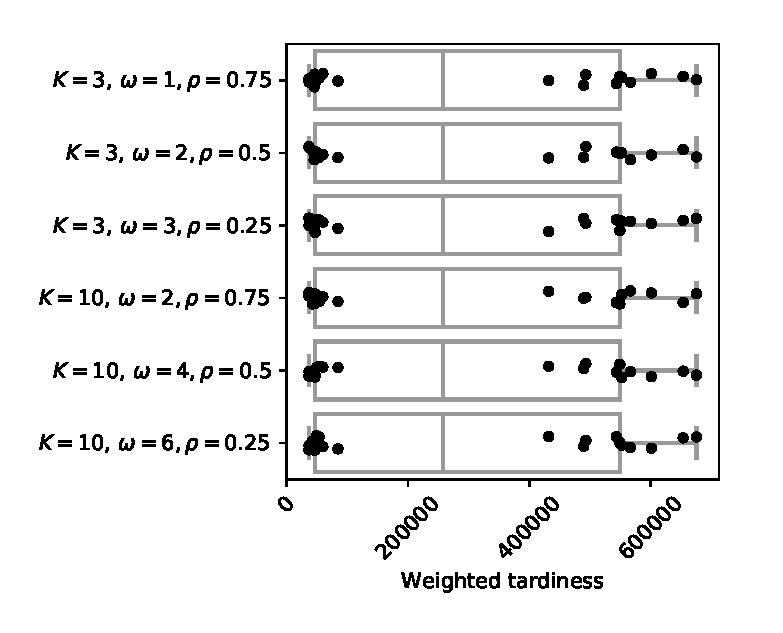
\includegraphics[width=0.7\textwidth]{RankBasedAS-params.eps}
	\caption{Evaluation of different parameters configurations for the
	Rank-based Ant System algorithm. All configurations gave identical
	solutions, for all problem instances.}
	\label{RankBasedAS-params}
\end{figure}

\begin{figure}
    \centering
    \begin{minipage}{.48\textwidth}
		\centering
		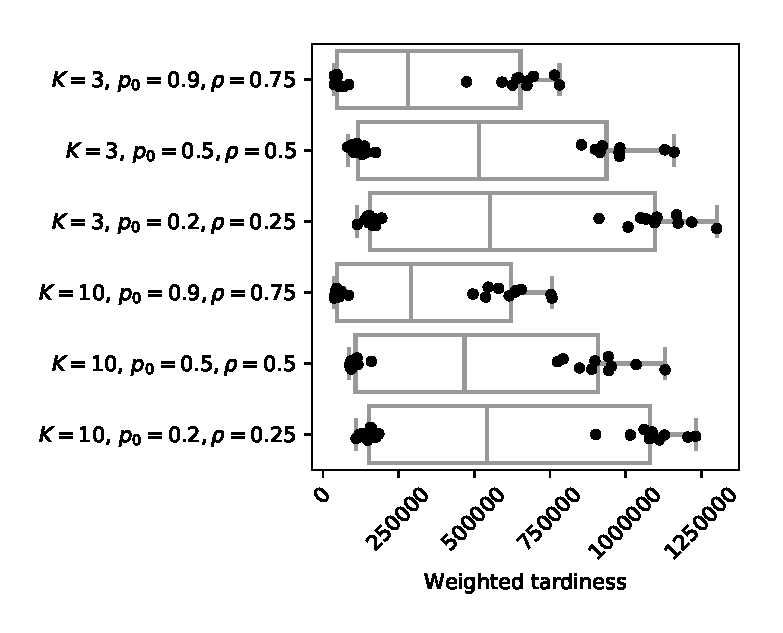
\includegraphics[width=1.1\textwidth]{MaxMinAS-params.eps}
		\caption{Evaluation of different parameters configurations for the Max-Min
		Ant System algorithm. The best performing configuration is using 3 or 10
		ants, with an exploitation probability of $p_0=0.9$, and a trail persistence
		factor $\rho=0.75$.}
		\label{MaxMinAS-params}
    \end{minipage}
    \hspace{0.02\textwidth}
    \begin{minipage}{.48\textwidth}
		\centering
		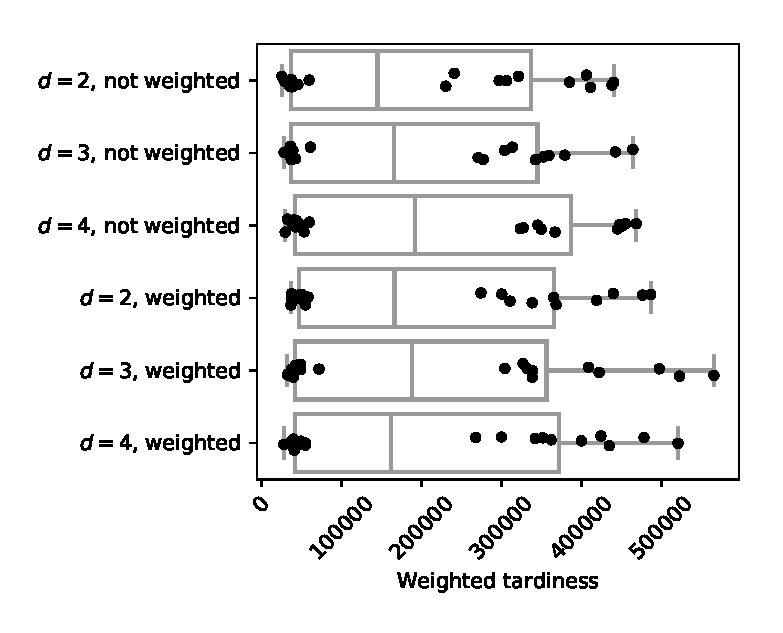
\includegraphics[width=1.1\textwidth]{IG_RLS-params.eps}
		\caption{Evaluation of different parameters configurations for the IG-RLS
		algorithm. The best performing configuration is to destruct-construct $d=2$
		jobs in the local search, with no weighting in the temperature calculation.}
		\label{IG_RLS-params}
    \end{minipage}
\end{figure}

The results of the performance assessment are given in figures
\ref{small-instances-results} and \ref{large-instances-results}. We separated
the results into two plots, since the magnitude of the numerical results is
different between the first 10 instances and the last 10 due to the different
number of jobs and machines. The IG-RLS performs consistently better than the
two AS approaches. RB-AS is better than MM-AS on large problem instances, but
show equivalent performances on small problem instances.

\begin{figure}
    \centering
    \begin{minipage}{.48\textwidth}
		\centering
		\includegraphics[width=1.1\textwidth]{small-instances-results.eps}
		\caption{Comparison of all three algorithms with best parameters. Only
		small instances are shown. The two ant system approaches show similar
		performances and are outperformed by the iterated search approach.}
		\label{small-instances-results}
    \end{minipage}
    \hspace{0.02\textwidth}
    \begin{minipage}{.48\textwidth}
		\centering
		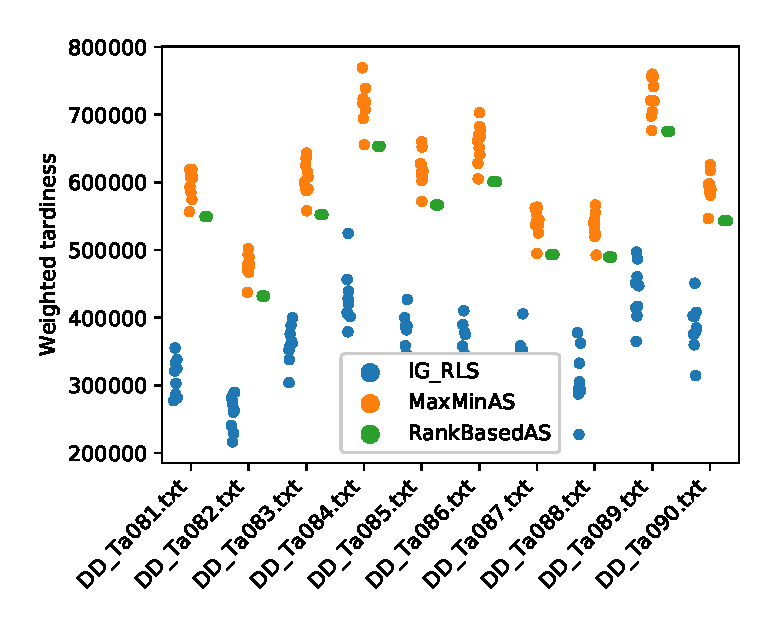
\includegraphics[width=1.1\textwidth]{large-instances-results.eps}
		\caption{Comparison of all three algorithms with best parameters. Only
		large instances are shown. The Rank-based approach performs as well as
		the best run of the Max-Min ant system. The iterated search clearly
		outperforms the two ant systems.}
		\label{large-instances-results}
    \end{minipage}
\end{figure}

\begin{table}
	\centering
	\begin{tabular}{lrrr}
		\toprule
		& RB-AS vs MM-AS & RB-AS vs IG-RLS & MM-AS vs IG-RLS \\
		\midrule
		\texttt{DD\_Ta051} & 0.95     & $<$ 0.01 & $<$ 0.01 \\
		\texttt{DD\_Ta052} & 1        & $<$ 0.01 & $<$ 0.01 \\
		\texttt{DD\_Ta053} & 0.20     & $<$ 0.01 & $<$ 0.01 \\
		\texttt{DD\_Ta054} & 0.84     & $<$ 0.01 & $<$ 0.01 \\
		\texttt{DD\_Ta055} & 0.09     & $<$ 0.01 &     0.01 \\
		\texttt{DD\_Ta056} & 1        & $<$ 0.01 & $<$ 0.01 \\
		\texttt{DD\_Ta057} & 1        & 0.32     & 0.36     \\
		\texttt{DD\_Ta058} & 0.20     & $<$ 0.01 & $<$ 0.01 \\
		\texttt{DD\_Ta059} & 0.20     & $<$ 0.01 & $<$ 0.01 \\
		\texttt{DD\_Ta060} & 1        & $<$ 0.01 & $<$ 0.01 \\
		\texttt{DD\_Ta081} & $<$ 0.01 & $<$ 0.01 & $<$ 0.01 \\
		\texttt{DD\_Ta082} & $<$ 0.01 & $<$ 0.01 & $<$ 0.01 \\
		\texttt{DD\_Ta083} & $<$ 0.01 & $<$ 0.01 & $<$ 0.01 \\
		\texttt{DD\_Ta084} & $<$ 0.01 & $<$ 0.01 & $<$ 0.01 \\
		\texttt{DD\_Ta085} & $<$ 0.01 & $<$ 0.01 & $<$ 0.01 \\
		\texttt{DD\_Ta086} & $<$ 0.01 & $<$ 0.01 & $<$ 0.01 \\
		\texttt{DD\_Ta087} & $<$ 0.01 & $<$ 0.01 & $<$ 0.01 \\
		\texttt{DD\_Ta088} & $<$ 0.01 & $<$ 0.01 & $<$ 0.01 \\
		\texttt{DD\_Ta089} & $<$ 0.01 & $<$ 0.01 & $<$ 0.01 \\
		\texttt{DD\_Ta090} & $<$ 0.01 & $<$ 0.01 & $<$ 0.01 \\
		\bottomrule
	\end{tabular}
	\caption{Double-sided p-values for the Wilcoxon rank-sum test on the results
	of each algorithms using Bonferroni correction. The IG-RLS outperforms
	clearly the two other algorithms, and RB-AS is better than MM-AS only on large
	problem instances.}
\end{table}


\section{Conclusion}
\label{sec:conclusion}


\bibliographystyle{splncs04}
\bibliography{report}

\end{document}
